\section{Resultados}
\label{Sec:6-resultados}

Os testes revelaram algumas necessidades adicionais do sistema, como a necessidade de manutenção periódica da aplicação na nuvem, assim como outras imperfeições que limitaram a exatidão do sistema. 

Porém os resultados abaixo foram positivos ao resultar em uma arquitetura escalável e modularizada, o que aumenta as possibilidades do sistema.

\subsection{Telas principais}

As telas principais estão descritas nas seções a seguir, com seu funcionamento descrito.

\subsubsection{Listagem de equipamentos}

A figura \ref{fig:telas-equipamentos-list} mostra a tela de gerenciamento dos equipamentos, onde o usuário pode listar, criar, alterar ou remover os equipamentos.

\begin{figure}[H]
\centering
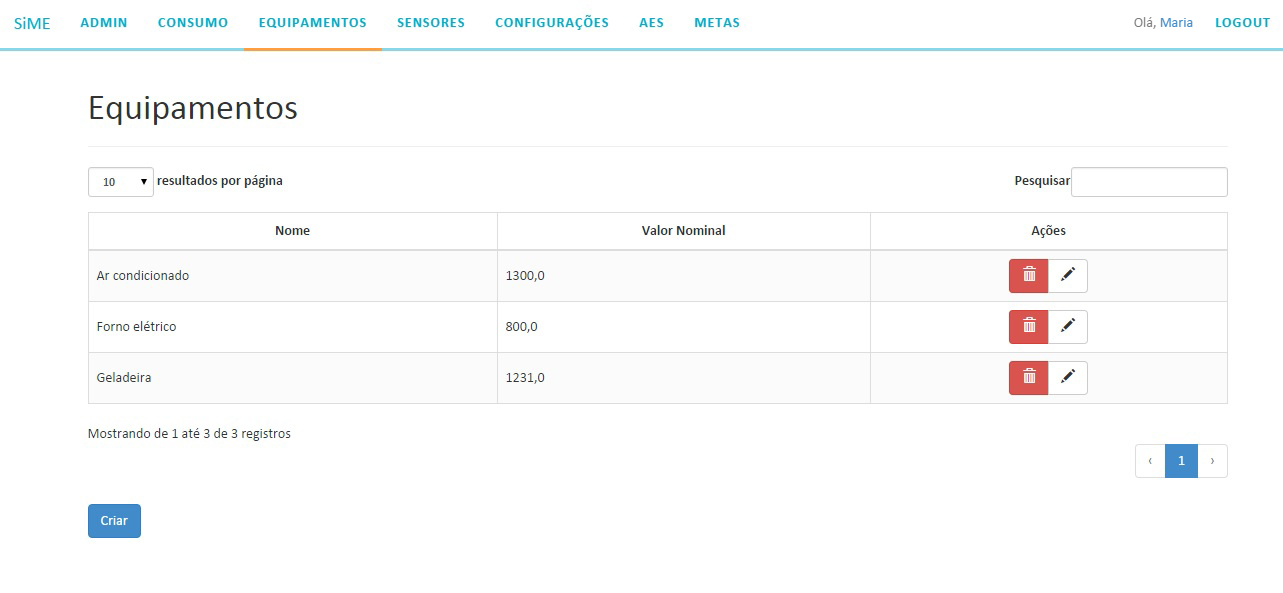
\includegraphics[width=1\textwidth]{figuras/equipamentos_list.jpg}
\caption{\label{fig:telas-equipamentos-list} Listagem de equipamentos}
\end{figure}

\subsubsection{Configurar sistema}

A figura \ref{fig:telas-config} mostra a tela de configuração, onde o usuário, através de ferramenta de \textit{drag and drop}, pode associar um sensor a um equipamento. Na mesma tela há a opção de escolher o tipo de renda, necessário para realizar a conversão do consumo em unidades monetárias através das taxas da AES.

\begin{figure}[H]
\centering
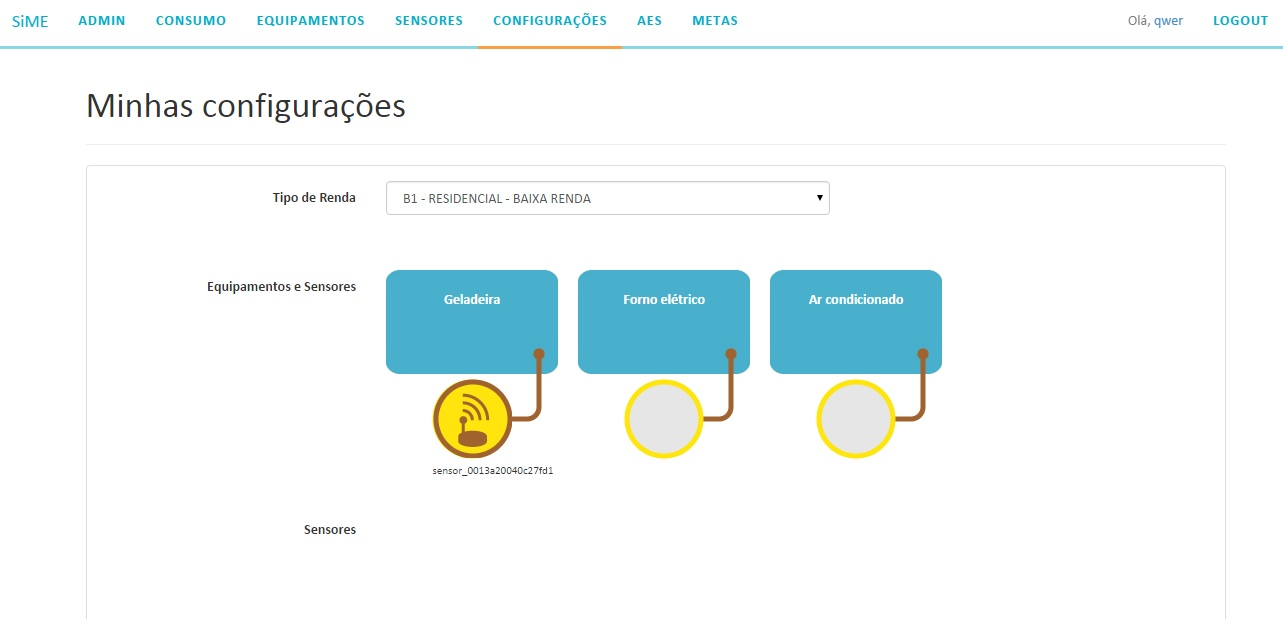
\includegraphics[width=1\textwidth]{figuras/configuracoes.jpg}
\caption{\label{fig:telas-config} Configurações}
\end{figure}

\subsubsection{Criar meta}

A figura \ref{fig:telas-metas-create} mostra a tela com formulário de criação de uma meta no sistema. Através dela o usuário pode criar metas de consumo em relação ao consumo obtido do mês anterior.

\begin{figure}[H]
\centering
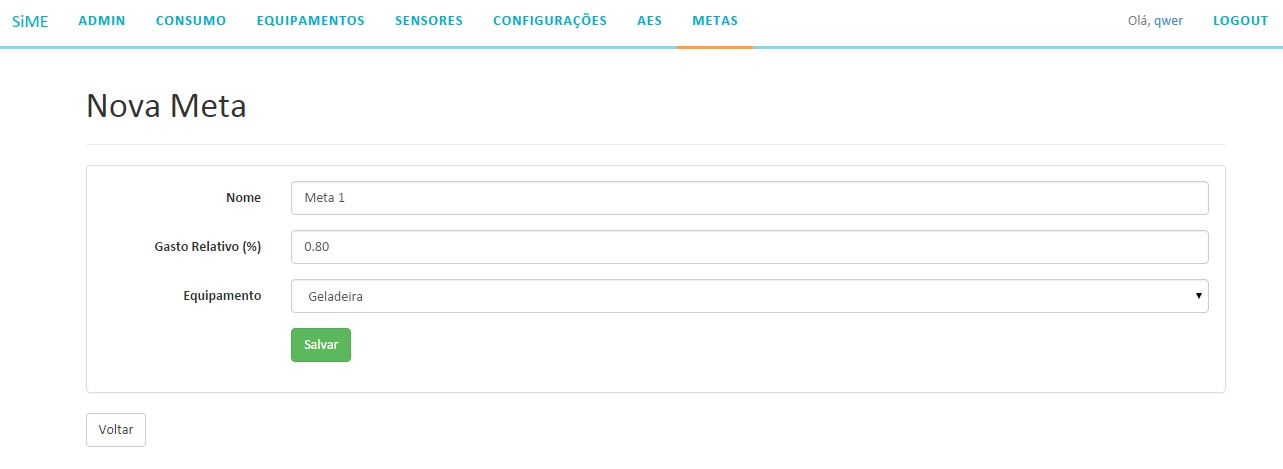
\includegraphics[width=1\textwidth]{figuras/meta.jpg}
\caption{\label{fig:telas-metas-create} Criar meta}
\end{figure}

\subsubsection{AES}

A figura \ref{fig:telas-aes} mostra a tela de visualização das taxas da AES. Ao clicar no botão de atualizar (logo abaixo do título), um robô da aplicação extrairá informações das tarifas no site da AES Eletropaulo e salvará no banco de dados, para posteriores consultas e cálculos. 

\begin{figure}[H]
\centering
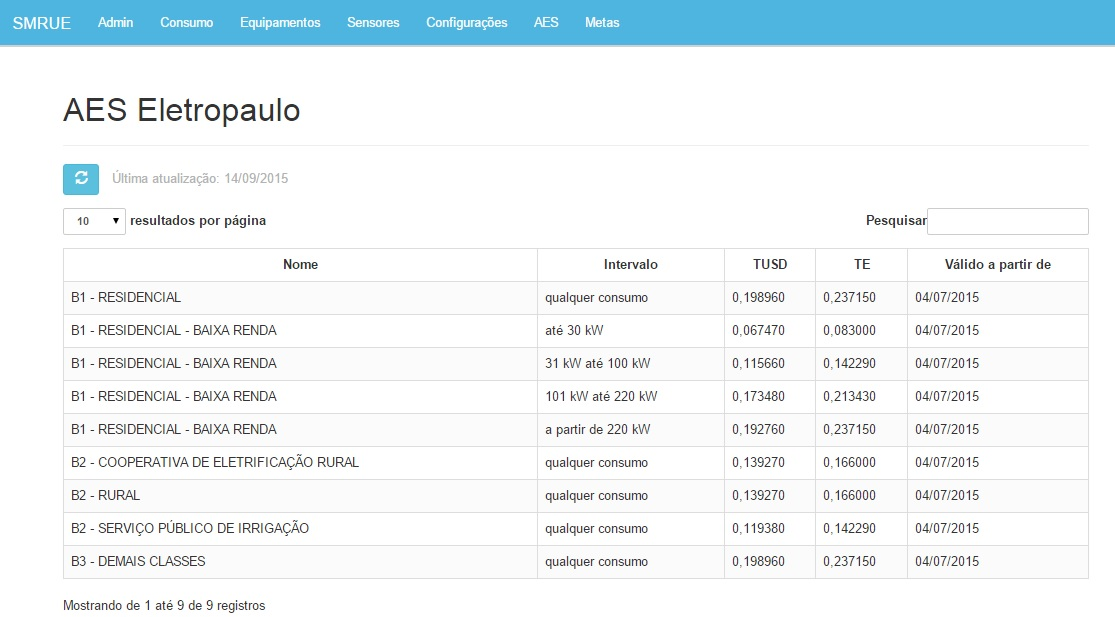
\includegraphics[width=1\textwidth]{figuras/aes.jpg}
\caption{\label{fig:telas-aes} AES}
\end{figure}

\subsubsection{Visualização dos dados medidos}

A figura \ref{fig:telas-grafico} mostra a página de consumo e o usuário possui algumas opções de exibição do gráfico. A primeira opção é a escolha do período do consumo. A aba Teste foi utilizada para fins de apresentação prática do projeto e mostra a potência consumida a cada 15 segundos. Já a aba Hora é utilizada para exibir a potência consumida a cada hora, dentro do intervalo de ano, mês/dia/hora escolhido pelo usuário. A aba Dia exibe a potência consumida por dia, dentro do intervalo de ano/mês/dia escolhido pelo usuário. A aba Mês exibe a potência consumida por Mês, dentro do intervalo de ano/mês escolhido pelo usuário.

Além do período, o usuário escolhe de quais equipamentos deseja visualizar a curva de consumo, podendo visualizar a curva com a soma de todos os equipamentos clicando em Somado. O gráfico resultante será apenas um, porém com todas as curvas escolhidas, assim como mostra a figura \ref{fig:telas-grafico}.  

A opção de integrar o gráfico, quando escolhida, realiza a conversão de cada ponto do gráfico de potência consumida para energia consumida acumulada desde o início do mês. Caso a opção de integrar o gráfico seja escolhida, a opção de incluir meta é habilitada. Caso esta última seja selecionada, o gráfico incluirá a curva da meta, que possui valor constante equivalente ao consumo desejado no mês atual, em relação ao mês anterior.

E por último, existe a opção da unidade de medida, que são Watt (W), Kilowatt (kW) e Reais (R\$). para W e kW, o gráfico ajusta o eixo vertical para grandeza escolhida. Já a unidade em Reais converte a energia consumida em kWh para Reais com base nas tarifas de energia da AES Eletropaulo, intervalo de energia consumido, tipo de renda do usuário e data de validade da tarifa.

Ao clicar no botão Fazer Gráfico, as opções escolhidas são computadas e o gráfico é renderizado.

\begin{figure}[H]
\centering
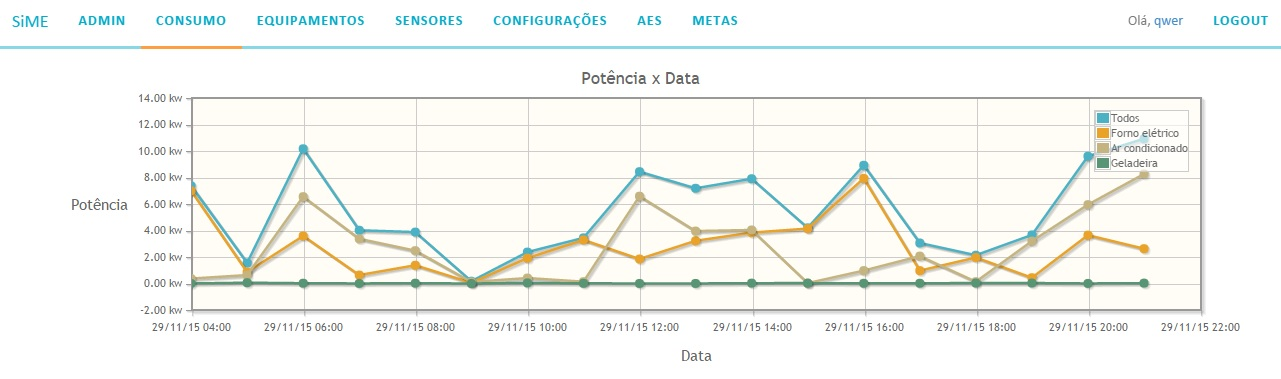
\includegraphics[width=1\textwidth]{figuras/consumo.jpg}
\caption{\label{fig:telas-grafico} Gráfico de consumo}
\end{figure}